\documentclass[a4]{article}
\usepackage{geometry}
\geometry{verbose,tmargin=2.5cm,bmargin=2.5cm,lmargin=3cm,rmargin=3cm}
\usepackage{amsmath,amssymb,amsthm}
\usepackage{graphicx}
\graphicspath{{graphics/}}
\usepackage[utf8]{inputenc}
\usepackage{fancyvrb}
\usepackage{hyperref}
\usepackage{lscape}
\usepackage{adjustbox}
\usepackage{verbatim}

\title{MultiFEBE \\ Tutorial 2: static analysis of a elastic cube with boundary elements}
\author{\'A.G. Vega-Artiles}
\date{June 2022}

\begin{document}

\maketitle

\begin{figure}[h]
	\centering
	\includegraphics{cube.eps}
	\caption{Problem layout.}
	\label{fig:layout}
\end{figure}

\section{Problem description}

In this second tutorial, a static analysis of an elastic cube is performed using the Boundary Element Method (BEM), i.e. boundary elements. Figure \ref{fig:layout} shows the geometry, required material properties and boundary conditions, where $E$ is the Young's modulus, $\nu$ is the Poisson's ratio, $L$ is the square side length and $P$ is the load. Note that self-weight is not considered. The analytical solution to this problem is easily obtained, which results in the following displacement and stress fields:

\begin{align}
u_1 &= \dfrac{(1+\nu)(1-2\nu)}{E(1-\nu)} P x_1 \\
u_2 &= u_3 = 0 \\
\sigma_{11} &= P \\
\sigma_{22} &= \sigma_{33} = \dfrac{\nu}{1-\nu}P \\
\sigma_{12} &= \sigma_{13} = \sigma_{23}= 0
\end{align}

from which it can be checked that tractions $t_i=\sigma_{ij}n_j$ ($n_j$ are the components of the outward unit normal components) obviously verify the boundary conditions. Displacement field is linear along $x_1$-direction and constant (null) along $x_2$ and $x_3$-direction. Also, the only non-null stresses ($\sigma_{11}$, $\sigma_{22}$ and $\sigma_{33}$) are constant. Therefore, numerical solution using linear or higher order elements must recover the analytical solution.

The problem is solved for $L=1$ $\mathrm{m}$, $E=1$ $\mathrm{N/m^2}$, $\nu=0.25$  and $P=1$ $\mathrm{N/m^2}$ and the results are the followings:

	$u_1 = 0.8\overline{3} x_1$ $\mathrm{N/m^2}$;
	$u_2 = u_3 = 0$;
	$\sigma_{11} = 1$ $\mathrm{N/m^2}$;
	$\sigma_{22} = \sigma_{33} = 0.\overline{3}$ $\mathrm{N/m^2}$;
	$\sigma_{12} = \sigma_{13} = \sigma_{23} = 0$.

\section{Pre-processing} 
Pre-processing in MultiFEBE consists of defining the geometry and mesh of the problem. There are three ways to do such definition: directly from the input file (mode = 0), from another file in the native format (mode = 1) or from another file in the Gmsh MSH file format version 2.2 (mode = 2) \cite{gmsh}. However, it is preferable to use a *.msh file for relatively large geometries, therefore, this is the syntax explained in the following subsections. Furthermore, as the problem will be solved using only the BEM formulation, the approaches explained in the previous section will be applied.      

\subsection{Gmsh format}
Gmsh \cite{gmsh, gmshweb} is a finite element mesh generator with its own language. The software allows to create the geometry in a “bottom-up” manner, going from the most basic elements (points) to the highest order elements (volumes) or in a “Constructive Solid Geometry” manner (boolean operations) or with a combination of methodologies. Gmsh also allows to define  the so-called “physical groups” which are unmodifiable entities that gather elementary entities as sole entities, where every entity must have a unique tag. On the other hand, the file containing all this geometric definition is the file *.geo whereas the mesh definition is in the file *.msh. 

\subsubsection{File *.geo}

The Gmsh language allows to define parameters to use later in the script and comments as every other programming language. 

In this example two parameters are defined: the square side length (L) and the mesh element size (es). Every point in the geometry can be specified by its coordinates (x y z) and the mesh element size to use there with the function "Point" and every straight line of the model is created with the function "Line" and its initial and final points. Then, every surface is  created with the function "Plane Surface" by setting its perimeter with the function "Line Loop" and the lines used to close the surface. Furthermore, with the function "Physical Surface" every surface is converted into a single entity or physical entity with its own name.  

It is worth noting that “if an expression defines a new entity, it is enclosed between parentheses but if an expression refers to a previously defined entity, it is enclosed between braces.” \cite{gmshweb}

Finally, the mesh generation, the element order and the *.msh file saving can also be specified with the expressions \textit{Mesh + mesh dimension}, \textit{SetOrder + element order} and \textit{Save + "name.msh"}, respectively.

The resulting *.geo file applied to the problem is the following:

\begin{Verbatim}
L = 1;  // Square side length
es = 1; // Element size

// Front Face
Point (1) = {0, 0, L, es};
Point (2) = {L, 0, L, es};
Point (3) = {L, L, L, es};
Point (4) = {0, L, L, es};
Line (1) = {1, 2};
Line (2) = {2, 3};
Line (3) = {3, 4};
Line (4) = {4, 1};
Line Loop (1) = {1, 2, 3, 4};
Plane Surface (1) = {1};
Physical Surface ("front", 1) = {1};

// Right Face
Point(5) = {L, 0, L, es};
Point(6) = {L, 0, 0, es};
Point (7) = {L, L, 0, es};
Point (8) = {L, L, L, es};
Line (5) = {5, 6};
Line (6) = {6, 7};
Line (7) = {7, 8};
Line (8) = {8, 5};
Line Loop (2) = {5, 6, 7, 8};
Plane Surface (2) = {2};
Physical Surface ("right", 2) = {2};

// Back Face
Point(9) = {L,  0, 0, es};
Point(10) = {0, 0, 0,  es};
Point (11) = {0, L, 0, es};
Point (12) = {L, L, 0, es};
Line (9) = {9, 10};
Line (10) = {10, 11};
Line (11) = {11, 12};
Line (12) = {12, 9};
Line Loop (3) = {9, 10, 11, 12};
Plane Surface (3) = {3};
Physical Surface ("back", 3) = {3};

// Left Face
Point(13) = {0, 0, 0, es};
Point(14) = {0, 0, L, es};
Point (15) = {0, L, L, es};
Point (16) = {0, L, 0, es};
Line (13) = {13, 14};
Line (14) = {14, 15};
Line (15) = {15, 16};
Line (16) = {16, 13};
Line Loop (4) = {13, 14, 15, 16};
Plane Surface (4) = {4};
Physical Surface ("left", 4) = {4};

// Top Face
Point(17) = {0, L, L, es};
Point(18) = {L, L, L, es};
Point (19) = {L, L, 0, es};
Point (20) = {0, L, 0, es};
Line (17) = {17, 18};
Line (18) = {18, 19};
Line (19) = {19, 20};
Line (20) = {20, 17};
Line Loop (5) = {17, 18, 19, 20};
Plane Surface (5) = {5};
Physical Surface ("top", 5) = {5};

// Bottom Face
Point(21) = {0, 0, L, es};
Point(22) = {0, 0, 0, es};
Point (23) = {L, 0, 0, es};
Point (24) = {L, 0, L, es};
Line (21) = {21, 22};
Line (22) = {22, 23};
Line (23) = {23, 24};
Line (24) = {24, 21};
Line Loop (6) = {21, 22, 23, 24};
Plane Surface (6) = {6};
Physical Surface ("bottom", 6) = {6};

// Mesh generation
Mesh 2;
SetOrder 1;
Save "t2.msh";
\end{Verbatim}

\begin{figure}[h]
	\centering
	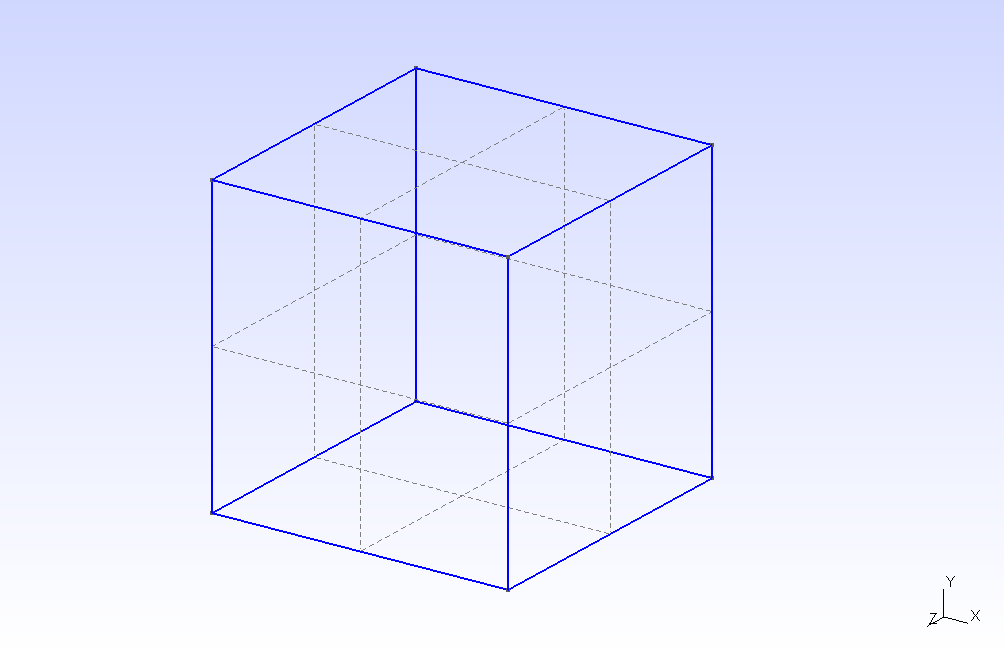
\includegraphics[scale = 0.3]{geometry.png}
	\caption{File *.geo. Geometry.}
	\label{fig:geometry}
\end{figure}

\subsubsection{File *.msh}
The *.msh file begins with a mandatory section about information of the file (MeshFormat) and following by the other sections. Here, three sections are used: the physical group names (PhysicalName), the nodes (Nodes) and the elements (Elements).

In the section "PhysicalName", all the physical entities of the model are defined. The first line
indicates the number of physical entities. Then, one line per physical entity indicating the physical dimension, the tag and the name.  
   
In the section "Nodes", all the nodes of the model are defined. The first line indicates the number of nodes. Then, one line per node indicating the identifier of the node and its coordinates (x y z).

In the section "Elements", all the elements of the model are defined. The first line indicates the number of elements. Then, one line per element indicating:

\begin{itemize}
	\item Element identifier.
	\item Type of element.
	\item Number of auxiliary tags.
	\item List of tags, where the two first auxiliary tag are mandatory, and corresponds to the identifier of the physical entity to which the element belongs and the second one is the identifier of the elementary model entity to which the element belongs. The rest of the tags are optional.
	\item A list of identifiers corresponding to the nodes of the element.
\end{itemize}

For example, in this case, an element with the identifiers 1 2 2 1 1 1 2 25 corresponds to:

\begin{itemize}
	\item 1: element 1.
	\item 2: type 2 (3-node triangle).
	\item 2: it has 2 auxiliary tags.
	\item 1: it belongs to the physical entity 1.
	\item 1: it belongs to the surface 1.
	\item 1, 2, 25: it connects the nodes 1, 2 and 25.
\end{itemize} 

Finally, the *.msh file can be obtain in  \textit{File $\to$ Export} or by following the instructions specified in the section \textit{File *.geo}.

The resulting *.msh file applied to the problem is the following:

\begin{Verbatim}
$MeshFormat
2.2 0 8
$EndMeshFormat

$PhysicalNames
6
2 1 "front"
2 2 "right"
2 3 "back"
2 4 "left"
2 5 "top"
2 6 "bottom"
$EndPhysicalNames

$Nodes
30
1 0 0 1
2 1 0 1
3 1 1 1
4 0 1 1
5 1 0 1
6 1 0 0
7 1 1 0
8 1 1 1
9 1 0 0
10 0 0 0
11 0 1 0
12 1 1 0
13 0 0 0
14 0 0 1
15 0 1 1
16 0 1 0
17 0 1 1
18 1 1 1
19 1 1 0
20 0 1 0
21 0 0 1
22 0 0 0
23 1 0 0
24 1 0 1
25 0.5 0.5 1
26 1 0.5 0.5
27 0.5 0.5 0
28 0 0.5 0.5
29 0.5 1 0.5
30 0.5 0 0.5
$EndNodes

$Elements
24
1 2 2 1 1 1 2 25
2 2 2 1 1 1 25 4
3 2 2 1 1 2 3 25
4 2 2 1 1 3 4 25
5 2 2 2 2 5 6 26
6 2 2 2 2 5 26 8
7 2 2 2 2 6 7 26
8 2 2 2 2 7 8 26
9 2 2 3 3 9 10 27
10 2 2 3 3 9 27 12
11 2 2 3 3 10 11 27
12 2 2 3 3 11 12 27
13 2 2 4 4 13 14 28
14 2 2 4 4 13 28 16
15 2 2 4 4 14 15 28
16 2 2 4 4 15 16 28
17 2 2 5 5 17 18 29
18 2 2 5 5 17 29 20
19 2 2 5 5 18 19 29
20 2 2 5 5 19 20 29
21 2 2 6 6 21 22 30
22 2 2 6 6 21 30 24
23 2 2 6 6 22 23 30
24 2 2 6 6 23 24 30
$EndElements
\end{Verbatim}

\begin{figure}[h]
	\centering
	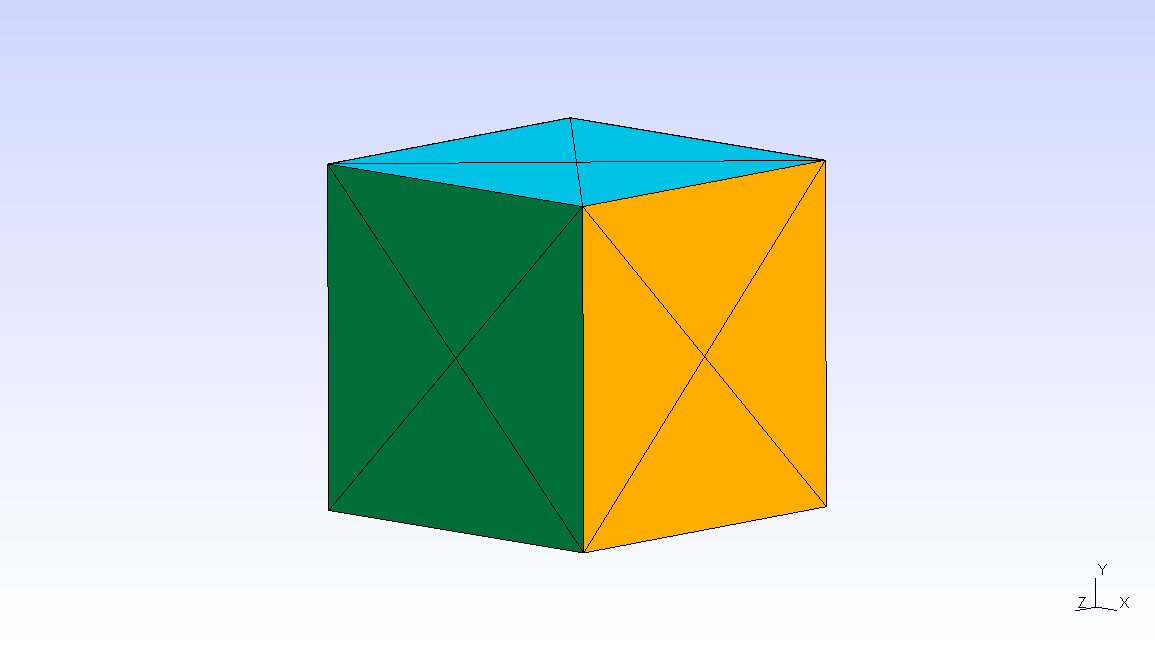
\includegraphics[scale = 0.3]{msh_file2.png}
	\caption{File *.msh. Mesh.}
	\label{fig:mesh}
\end{figure}

\section{Solving}
Solving in MultiFEBE consists of running the software by specifying several options in the following sections\footnote{See reference manual.}: [problem], [settings], [materials], [boundaries], [regions] and [conditions over the boundaries].

The first part to configurate is the problem definition in the section [problem]. This example is a 3D static mechanical problem.  

\begin{Verbatim}	
[problem]
n = 3D
type = mechanics
analysis = static
\end{Verbatim}

Next step is to configurate the mesh. In this case, a mesh from \textit{Gmsh} will be used so that it is necessary to write the option number 2 and the document name obtained from it in the section [settings]. However, if the mesh were going to be read from the input file, it would require to write the sections [nodes], [elements] and [parts] instead.

\begin{Verbatim}	
[settings]
mesh_file_mode = 2 "t2.msh"
\end{Verbatim}

As the problem has just one material, the section [materials] will need two lines: a first line for the number of materials in the model and a second line for the properties such as tag, name, E and $\nu$.

\begin{Verbatim}	
[materials]
1
1 elastic_solid E 1. nu 0.25
\end{Verbatim}

In the section [boundaries] it is necessary to specify the number of boundaries in the first line and a line per boundary by indicating the boundary identifier,
the identifier of the part that discretize it, and finally the boundary class. In this example there are 6 boundaries: boundary 1 is the part 1 of the mesh, boundary 2 the part 2, boundary 3 the part 3, boundary 4 the part 4, boundary 5 the part 5 and boundary 6 the part 6 and all of them are ordinary boundaries.

\begin{Verbatim}	
[boundaries]
6
1 1 ordinary
2 2 ordinary
3 3 ordinary
4 4 ordinary
5 5 ordinary
6 6 ordinary
\end{Verbatim}

The format of the [regions] section consists of a first line indicating the number of regions (1). Furthermore, for each region there must be a block of data consisting of several lines of data. The first one is the region identifier and the region class (discretization method) (1 be). As the region is a BE region, then the second line indicates the number of boundaries and a list of boundaries (6 1 2 3 4 5 6). The third line defines the material (material 1). Then, for a BE region, the fourth line defines the number and a list of BE body loads (0).

\begin{Verbatim}	
[regions]
1

1 be
6 1 2 3 4 5 6
material 1
0
\end{Verbatim}

In the section [conditions over be boundaries] all boundaries will be specify in global coordinates because they are planar and their normal vectors are parallel to one of the global axes. As a 3D problem, there are three lines for every boundary: a first line for the "x" direction, the second one for the "y" direction and the third one for the "z" direction, where the first number of every line indicates the type of condition (here 0 for displacement and 1 for traction) and the second one its value.

\begin{Verbatim}	
[conditions over be boundaries]
boundary 1: 1 0.
            1 0.
            0 0.
boundary 2: 1 1.
            1 0.
            1 0.
boundary 3: 1 0.
            1 0.
            0 0.
boundary 4: 0 0.
            1 0.
            1 0.
boundary 5: 1 0.
            0 0.
            1 0.
boundary 6: 1 0.
            0 0.
            1 0.
\end{Verbatim}

The whole script applied to the problem is the following:

\begin{Verbatim}
[problem]
n = 3D
type = mechanics
analysis = static

[settings]
mesh_file_mode = 2 "t2.msh"

[materials]
1
1 elastic_solid E 1. nu 0.25

[boundaries]
6
1 1 ordinary
2 2 ordinary
3 3 ordinary
4 4 ordinary
5 5 ordinary
6 6 ordinary

[regions]
1

1 be
6 1 2 3 4 5 6
material 1
0

[conditions over be boundaries]
boundary 1: 1 0.
            1 0.
            0 0.

boundary 2: 1 1.
            1 0.
            1 0.

boundary 3: 1 0.
            1 0.
            0 0.

boundary 4: 0 0.
            1 0.
            1 0.

boundary 5: 1 0.
            0 0.
            1 0.

boundary 6: 1 0.
            0 0.
            1 0.           
\end{Verbatim}

\section{Post-processing}

\subsection{Nodal solutions file (*.nso)}

This output file is similar to the file for the 2D example\footnote{See Tutorial 1.}, but with more columns due to the z dimension. 

\subsection{Stress resultant solutions (*.tot)}

This output file is a plain text file containing the resultant  displacement, rotation, forces and moments of the centroid of every boundary element. The file starts with a set of header lines whose first character is "$\#$" (a comment line in GNU/Linux environments), describing the file and the meaning of the main data columns. 

\begin{Verbatim}
# Program      : multifebe
# Version      : 0.6
# File_format  : tot
# Specification: 1
# Input_file   : t2.dat
# Description  : 
# Timestamp    : 2022-05-24 19:20:59.188

# Columns  Description
# 1-3      Region id, class and type.
# 4-6      Boundary id, class and face.
# 7-9      Reference point
# 10-12    Resultant displacements along x1, x2 and x3
# 13-15    Resultant rotations in x1, x2 and x3 directions with respect to the reference point
# 16-18    Resultant forces along x1, x2 and x3
# 19-21    Resultant moments in x1, x2 and x3 directions with respect to the reference point
\end{Verbatim}

The file for the current example is the following:

\begin{Verbatim}
Columns 1-9
1__2__3__4__5__6____7__________________________8__________________________9_______________________
1  1  2  1  1  1    0.0000000000000000E+000    0.0000000000000000E+000    0.0000000000000000E+000 
1  1  2  2  1  1    0.0000000000000000E+000    0.0000000000000000E+000    0.0000000000000000E+000 
1  1  2  3  1  1    0.0000000000000000E+000    0.0000000000000000E+000    0.0000000000000000E+000
1  1  2  4  1  1    0.0000000000000000E+000    0.0000000000000000E+000    0.0000000000000000E+000
1  1  2  5  1  1    0.0000000000000000E+000    0.0000000000000000E+000    0.0000000000000000E+000  
1  1  2  6  1  1    0.0000000000000000E+000    0.0000000000000000E+000    0.0000000000000000E+000  

Columns 10-12
10_________________________11_________________________12_________________________
 416.6665124818034194E-003  -21.7024668712401838E-009    0.0000000000000000E+000  
 833.3332552543941674E-003  -33.4323049126867974E-009   89.2479633341829967E-009  
 416.6667054423257577E-003   40.8574092343643430E-009    0.0000000000000000E+000   
   0.0000000000000000E+000    2.2524860476320668E-009    2.9071411468239618E-009 
 416.6666696645033863E-003    0.0000000000000000E+000   44.0662267443331586E-009   
 416.6666093799233361E-003    0.0000000000000000E+000  -25.5497694805328682E-009    

Columns 13-15
13_________________________14_________________________15_________________________
  15.2971017006141144E-009  302.9093621814738513E-003 -308.8234562630653990E-003    
 149.1666871671048083E-009  302.9093607072384509E-003 -302.9094707058440639E-003    
   0.0000000000000000E+000    0.0000000000000000E+000 -308.8235240258003778E-003  
-646.6494794654632685E-012    0.0000000000000000E+000    0.0000000000000000E+000 
  31.5797144098362004E-009  308.8234975533534765E-003 -302.9094669326845568E-003   
   0.0000000000000000E+000  308.8235102637851281E-003    0.0000000000000000E+000    


Columns 16-18
16_________________________17_________________________18_________________________
   0.0000000000000000E+000    0.0000000000000000E+000  333.3332709461450660E-003  
   1.0000000000000000E+000    0.0000000000000000E+000    0.0000000000000000E+000    
   0.0000000000000000E+000    0.0000000000000000E+000 -333.3332716617732894E-003 
-999.9999479918649792E-003    0.0000000000000000E+000    0.0000000000000000E+000    
   0.0000000000000000E+000  333.3332477869328514E-003    0.0000000000000000E+000 
   0.0000000000000000E+000 -333.3332443552787794E-003    0.0000000000000000E+000  
  
Columns 19-21
19_________________________20_________________________21_________________________
 166.6666343762666647E-003 -166.6666073691435712E-003    0.0000000000000000E+000
   0.0000000000000000E+000  500.0000000000000000E-003 -500.0000000000001110E-003
-166.6666224357595538E-003  166.6666319121406503E-003    0.0000000000000000E+000
   0.0000000000000000E+000 -499.9999707659261161E-003  499.9999745497061832E-003
-166.6666205682695856E-003    0.0000000000000000E+000  166.6666103287823275E-003
 166.6666316894805655E-003    0.0000000000000000E+000 -166.6666059412922896E-003
\end{Verbatim}

\subsection{Gmsh results file (*.pos)}

This output file is similar to the file for the 2D example\footnote{See Tutorial 1.}, but with more columns due to the z dimension. 

\begin{figure}[h]
	\centering
	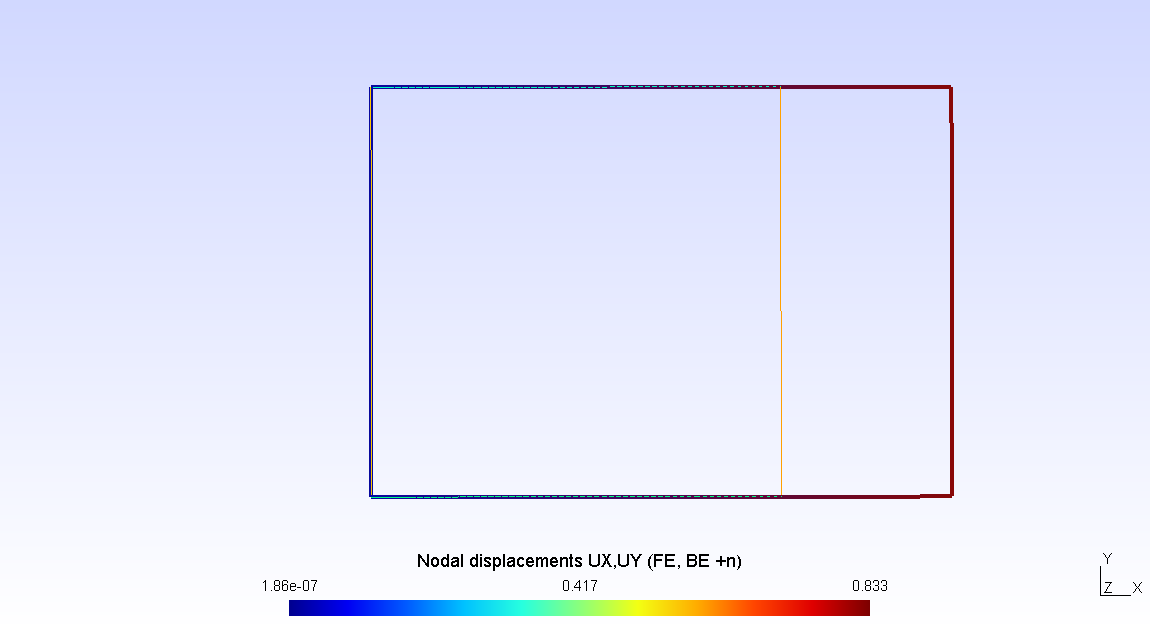
\includegraphics[scale = 0.5]{displacement.png}
	\caption{File *.pos. Nodal displacement results.}
	\label{fig:displacement}
\end{figure}

\begin{figure}
	\centering
	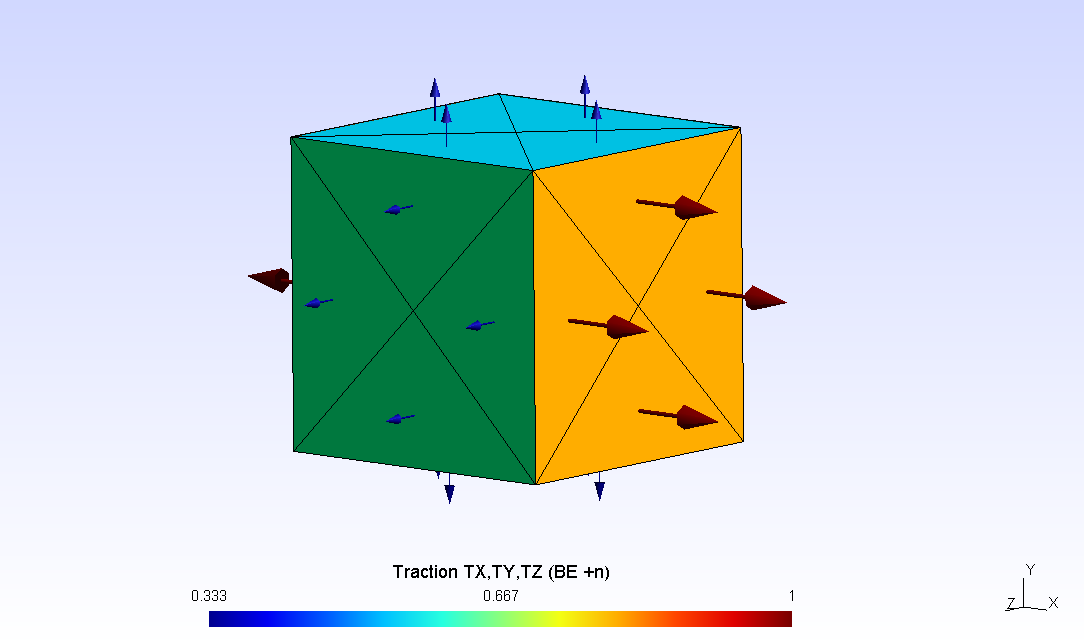
\includegraphics[scale = 0.5]{traction.png}
	\caption{File *.pos. Traction results.}
	\label{fig:traction}
\end{figure}

\begin{figure}
	\centering
	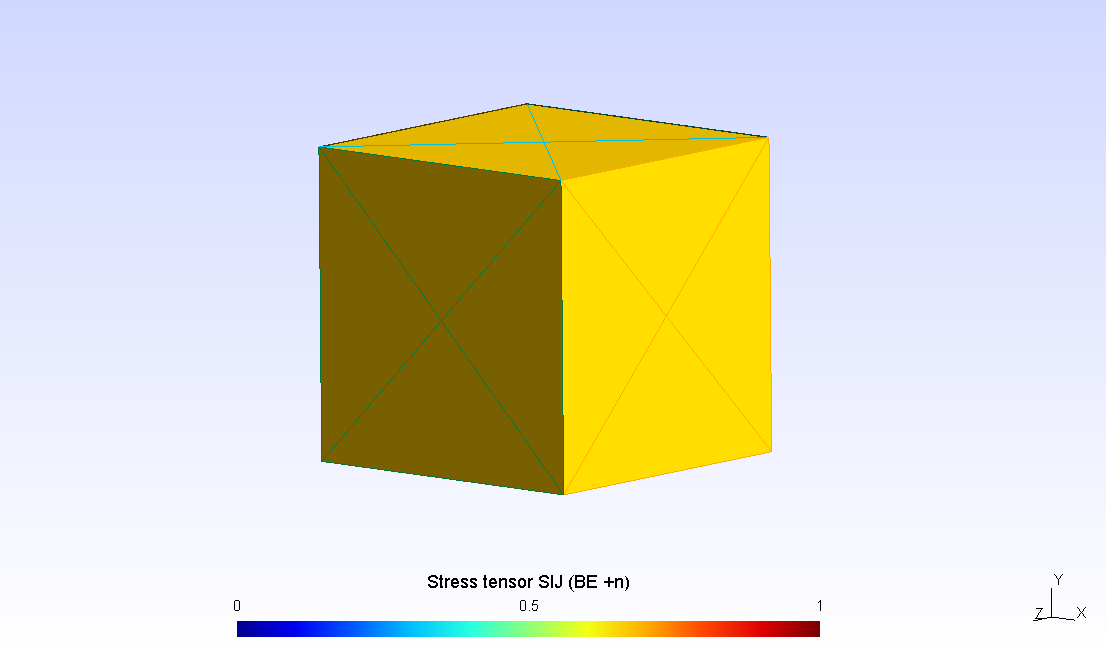
\includegraphics[scale = 0.5]{stress.png}
	\caption{File *.pos. Stress tensor results.}
	\label{fig:stress}
\end{figure}

\begin{thebibliography}{99}
	
	\bibitem{gmsh} C. Geuzaine and J.-F. Remacle, "Gmsh: a three-dimensional finite element mesh generator with built-in pre- and post-processing facilities." \emph{Int. J. Numer. Methods Eng.}, Volume 79, Issue 11, pages 1309--1331, (2009)
	
	\bibitem{gmshweb} C. Geuzaine and J.-F. Remacle, "Gmsh." \url{http://gmsh.info/}
	
\end{thebibliography}

\end{document}
